\chapter{Identity, Communication, and Data Architecture}
\label{chap:identity-data}
% Traceability: ADR-002 ADR-003 ADR-006

Every active board is an independent network device. The host must know which board performs each instrument role, configure it safely, supervise it while armed, and receive its data. This must still work when a board is replaced or its network settings are wrong.

The architecture separates persistent service information from normal operation. UART provides local commissioning and recovery. Ethernet provides operational control, status, supervision, and science data. The host owns the instrument inventory.

\section{Direct Host-to-Board Communication}

Each active board has its own Ethernet endpoint. The host communicates directly with the main board, every function board, and every bridge board. Function boards do not send ordinary traffic through the main board, and they do not command one another.

The main board is one endpoint among the others. It receives system coordination requests, such as arm, disarm, clear, and acquisition timing requests. A video board receives its own configuration and sends its own science data. A clock or bias board receives the settings for its local function.

This direct model avoids two bottlenecks. Main does not need to process all board control traffic, and it does not need to carry the combined data rate of every video board. Communication capacity can grow with the installed boards and the instrument network.

Figure~\ref{fig:communication-ownership} shows the communication ownership and the separate UART service path.

\begin{figure}[htbp]
  \centering
  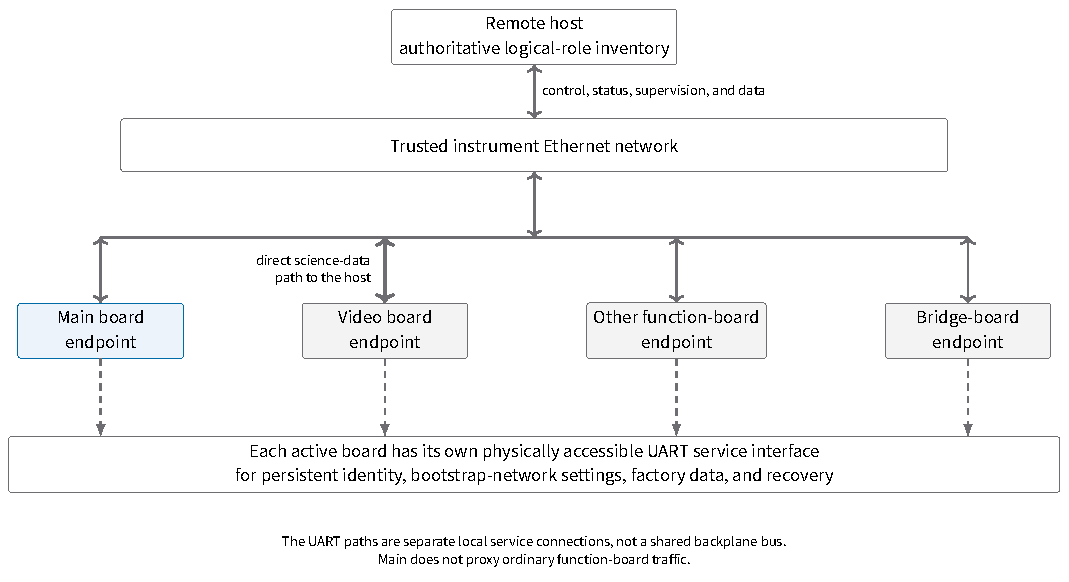
\includegraphics[width=\textwidth]{figures/generated/communication_ownership.tikz.pdf}
  \caption{Every active board is a direct Ethernet endpoint. Each also has its own local UART service interface for persistent commissioning and recovery.}
  \label{fig:communication-ownership}
\end{figure}

The architecture does not require one physical switch arrangement. Boards may connect directly or through suitable network switches. The instrument ICD defines the topology and verifies that each link has enough capacity for its control, telemetry, supervision, configuration, and acquisition traffic.

\section{Information and Configuration}

Not all board information should be stored or changed in the same way. Table~\ref{tab:information-lifetime} groups the main information classes by ownership, channel, and lifetime.

\begin{table}[htbp]
\centering
\small
\begin{tabularx}{\textwidth}{@{}>{\bfseries\raggedright\arraybackslash}p{0.20\textwidth}>{\raggedright\arraybackslash}p{0.25\textwidth}>{\raggedright\arraybackslash}p{0.22\textwidth}>{\raggedright\arraybackslash}X@{}}
\toprule
Information & Owner or source & Normal channel & Lifetime \\
\midrule
Board identity and bootstrap network & Board persistent storage; commissioned through service tools & UART service interface & Persists across reset and power loss \\
Factory calibration or trim & Board persistent storage and manufacturing records & UART service interface & Persists across reset and power loss \\
Firmware version & Active firmware image & Ethernet normally; UART during service & Describes the running image \\
Operational settings & Host sends values to the board & Ethernet & Current boot session \\
Sequencer payload & Host transfers to the sequencer board & Reliable ICD-defined host transfer & Current boot session; readiness is cleared by reset or power loss \\
Diagnostics and telemetry & Board monitoring and retained evidence & Ethernet normally; UART for recovery & Observation; selected evidence may remain until recovery \\
Science data & Video function board & Direct board-to-host data path & Acquisition product managed by the host system \\
Instrument inventory & Remote host & Host configuration and commissioning records & Persists independently of any one controller board \\
\bottomrule
\end{tabularx}
\caption{Information classes use channels and lifetimes that match their purpose.}
\label{tab:information-lifetime}
\end{table}

This separation prevents an ordinary operational command from silently changing the identity or future network behavior of a board. It also prevents old detector settings from returning automatically after a reset.

\subsection{Operational Configuration}

The host sends normal operating values over Ethernet while the board is safely disarmed. The board validates the values before applying them. The communication and board ICDs define which writes are allowed in each state and how invalid requests are reported.

Operational values are volatile. Reset or power loss restores safe defaults. Fault recovery and ordinary arm or disarm cycles do not automatically erase valid settings from the current boot session.

This behavior supports efficient recovery without treating potentially stale values as permanent board configuration. A board that lost or invalidated part of its operational state reports Not Ready until the host restores what is needed.

\subsection{Sequencer Transfer and Readiness}

Sequencer payloads are loaded only while safely disarmed. The transfer uses a reliable protocol defined by the applicable ICD. A sequencer board remains Not Ready until the host explicitly completes the transaction.

If accepted sequencer content is later modified, readiness is cleared again. Reset or power loss also clears sequencer readiness. A normal fault clear or arm/disarm cycle does not have to erase a valid payload unless the board's local behavior invalidated it.

The readiness indication confirms completion of the host loading transaction. The architecture does not require or prohibit an additional hash, content signature, or attestation check. Those mechanisms may be added by the board or instrument specification.

\section{Service, Identity, and Board Replacement}

Ethernet cannot be the only way to repair Ethernet configuration. A stale static address, incorrect bootstrap setting, or damaged operational image could make a board unreachable through its normal network path.

Every active board therefore provides a physically accessible UART service interface. It supports commissioning, allowed persistent-data access, fallback diagnostics, and recovery when normal Ethernet startup fails.

The UART connection is local to each board. It is not a shared backplane inventory bus. This keeps recovery available without adding another multi-board addressing system.

The communication ICD defines the electrical standard, connector, framing, request and response behavior, validation, and recovery entry. The architecture only requires that the service path remain accessible and independent of normal network reachability.

Interrupted persistent-data writes must not create a partially valid record. The board hardware and firmware designs choose the storage technology, validation method, redundancy, and atomic update method.

\subsection{Persistent Board Identity}

Each active board provides the persistent information needed to identify and commission it. Where applicable, this includes:

\begin{itemize}
  \item a unique MAC address;
  \item a unique serial or board identifier;
  \item board type and hardware revision;
  \item bootstrap IP information when static addressing is used; and
  \item required manufacturing calibration or trim data.
\end{itemize}

Software version is not stored as board identity. It is reported by the active firmware image. This allows the host to distinguish the physical board from the software currently running on it.

Normal detector biases, clock settings, timing values, enable masks, acquisition settings, and sequencer content are not persistent identity. They are operational values loaded for the current session.

Ethernet does not modify persistent board storage. Changes to identity, bootstrap settings, or factory information use the controlled UART service path.

\subsection{Host-Owned Logical Inventory}

Physical slot position is not the operational identity of a board. A controller may have different slot populations, and a bridge may extend the system to another backplane. Tying a logical role only to a slot would make replacement and topology changes difficult to manage.

The host owns the authoritative mapping:

\begin{center}
logical instrument role $\longleftrightarrow$ board capability and revision $\longleftrightarrow$ network endpoint $\longleftrightarrow$ MAC and serial identity
\end{center}

At startup, the host checks that each expected endpoint reports the expected identity and capability. A network response alone is not enough. The wrong board type at a reachable address must not be accepted as the required instrument function.

Slot information may still help a technician locate hardware, and an identification light or discovery tool may assist commissioning. Neither replaces the host inventory.

The main board does not need this complete function-board inventory to distribute shared electrical signals. It provides timing and coordination to the supported interfaces independently of the logical role assigned by the host.

\subsection{Replacing a Board}

A replacement board is commissioned in two deliberate steps.

First, a technician uses the board's UART service interface to verify its physical identity and set permitted bootstrap-network information. Second, the host inventory is updated to map the intended logical role to the replacement board's identity and endpoint.

The host then verifies the new mapping during startup and loads the required operational settings. Copying an old IP address is not enough, because the serial identity, hardware revision, or capability may differ.

The architecture does not define a complete service procedure. It defines the information and independent recovery path needed for a safe procedure to be written.

\section{Supervision and Science Traffic}

While armed, every active board requires a valid host interaction within a bounded interval. The interaction must prove communication in both directions. A board that only sends unsolicited data cannot know whether the host still receives or responds to it.

A host status request and board response can provide both acquisition-time health visibility and the qualifying supervision exchange. This demonstrates communication activity, not correct operation of every part of the host application. Measurements help the host diagnose conditions; protection requiring a timely local response must not depend on the host reading telemetry and sending a stop command.

The architecture does not mandate a separate heartbeat message. Telemetry, a heartbeat, an acknowledgement, data credit, or another bidirectional operation may qualify. The communication ICD selects the operation, cadence, retries, response, and timeout.

Chapter~\ref{chap:lifecycle} describes the armed timeout and fault response.

The implementation is verified at maximum supported traffic. A full data queue or a busy acquisition task must not delay the qualifying interaction without bound.

\subsection{Science Data Goes Directly to the Host}

Each video function board sends acquisition data directly to the remote host over its own network endpoint. There is no acquisition-data bus on the backplane, and the main board never carries science data.

The video-board and system ICDs define link rate, transport, framing, integrity checks, buffering, flow control, and reconnect behavior. The architecture does not choose TCP, another transport, a frame format, or a universal Ethernet speed. A board may use 100 Mb/s, 1 Gb/s, or another supported capacity according to its application. The application defines data products and rates, local processing or reduction, and buffering, with capacity verified at maximum supported load while preserving host supervision.

Using one board endpoint for both control and data avoids a second connector and physical link before measurements show that one is needed. The link budget must include maximum science traffic together with control, status, and supervision traffic.

If a specific instrument cannot meet its measured data requirement with that link, its ICD and design may add a dedicated data link. The direct board-to-host ownership and host-supervision rules remain unchanged.

\subsection{Data Overrun Is Not Automatically a Safety Fault}

If the network or host cannot accept data fast enough, a video board may overrun a buffer or lose part of an acquisition. This damages data quality, but it does not by itself mean that detector interface electronics are unsafe.

The board reports enough information for the host to identify the affected frames or acquisition. The transport follows its ICD-defined recovery behavior. The board does not pull \texttt{OK} low solely because data was lost.

Host supervision remains independent. If the board cannot complete the required bidirectional host interaction within the allowed armed interval, the supervision timeout still trips the controller. Local buffering and task scheduling must be sized and verified so maximum acquisition traffic does not hide this timeout path.

\section{Trusted Instrument-Network Boundary}

The standard architecture assumes a physically or logically isolated instrument network with trusted peers. This is a deployment condition, not a statement that Ethernet traffic is safe on any open network.

An instrument that cannot provide this boundary adds authentication or other controls in its deployment and communication specifications. Message-integrity checks may also be used where they improve reliability, independently of authentication.

A complete cybersecurity design depends on the observatory network, operating environment, update process, and threat model. Those details are outside this architecture handbook.

\medskip
\noindent\textit{Chapter sources:} ADR-002 defines persistent identity, UART recovery, host-owned inventory, operational configuration, direct board endpoints, and sequencer readiness. ADR-003 defines legal operating states and supervision consequences. ADR-006 defines direct acquisition-data ownership and overrun behavior.
